\documentclass{book}

\usepackage[shortsuper,hacm,ltfont]{common/uruwi}

\newcommand{\lname}{Middle Rymakonian}

\title{lek-\bs{}tsaro-ma sil lek-ma sil se\^otxe-\bs{}ri\^umako}
\author{uruwi}

\begin{document}

\pagecolor{Thistle!25}

\begin{titlepage}
    \makeatletter
    \begin{center}
        {\color{Orchid} \hprule \vspace{1.5ex} \\}
        {\Huge \ltfont \textcolor{Plum}{LKe\bs{}TSxaRMoa SL LKeMa SL STfXe\bs{}RMyaKo}\\}
        {\large \kardinal \textcolor{Purple}{\@title} \\}
        {\large \textit{\lname}, the language of \textit{Rymako} \\}
        {\color{Orchid} \hprule \vspace{1.5ex} \\}
        % ----------------------------------------------------------------
        \vspace{1.5cm}
        {\Large\bfseries \@author}\\[5pt]
        %uruwi@protonmail.com\\[14pt]
        % ----------------------------------------------------------------
        \vspace{2cm}
        {\Large\textlt{IVvoQMxeBPieLBxf TXxeKy}} \\
        \textkardinal{f\^ho\^e.on\^g-mebi-pelbe\^o txeki\^u} \\[5pt]
        \emph{A complete grammar}\\[2cm]
        %{in partial fulfilment for the award of the degree of} \\[2cm]
        %\tsc{\Large{{Doctor of Philosophy}}} \\[5pt]
        %{in some subject} \vspace{0.4cm} \\[2cm]
        % {By}\\[5pt] {\Large \sc {Me}}
        \vfill
        % ----------------------------------------------------------------
        %\includegraphics[width=0.19\textwidth]{example-image-a}\\[5pt]
        %{blah}\\[5pt]
        %{blahblah}\\[5pt]
        %{blahblah}\\
        \vfill
        {\@date}
    \end{center}
    \makeatother
\end{titlepage}

\pagecolor{Thistle!15}

\begin{center}
    \textit{Dedicated to Gufferdk.}
\end{center}

\begin{verbatim}
Branch: canon
Version: 0.1
Date: 2017-12-22 (29 dia len)
\end{verbatim}

(C)opyright 2017 Uruwi. See README.md for details.

\tableofcontents

\section{Introduction}

\chapter{Phonology and orthography}

\section{Phoneme inventory}

\lname{} underwent several sound changes from Lek-Tsaro, in the following order:

\begin{alignat*}{2}
  % \alpha &\rightarrow \omega &\quad(\lambda \blacklozenge \rho) &\quad[\Gamma]
  \text{s} &\rightarrow \text{s͎} &\quad(\blacklozenge \{\text{w}, \text{j}, \text{u}, \text{y}\}) &\quad \textit{NB this is a whistled sibiliant.} \\
  \text{ŋ} &\rightarrow \text{ɲ} &\quad(\square \blacklozenge) \\
  \text{θx} &\rightarrow \text{θ} &\quad\lnot(\blacklozenge \square) [\chi = \emptyset] \\
  C_1[+fr] &\rightarrow C_1[+v] &\quad(V_1 \blacklozenge V_2) \\
  \text{ɹ} &\rightarrow \text{z} &\quad(V_1 \blacklozenge V_2) \\
  \{\text{y̜}, \text{u̜}\} &\rightarrow \text{ʉ̜} \\
  V_1[+r] &\rightarrow V_1[-r] \\
  \text{k} &\rightarrow \text{c} &\quad (\blacklozenge \text{i}) \\
  \text{t} &\rightarrow \text{tʃ} &\quad (\blacklozenge \text{i}) \\
  \text{r} &\rightarrow \text{ɾ} \\
\end{alignat*}

Thus \lname{} has the following phoneme inventory:

\begin{table}[h]
  \caption{The consonants of \lname.}
  \centering
  \begin{tabular}{l|llllll}
      & Bilabial & Dental & Alveolar & Palatal & Velar & Glottal \\
      \hline
      Nasal & m & & n & ɲ & ŋ & \invalid \\
      Plosive & p b & & t d & c ɟ & k ɡ & ʔ \\
      Fricative & f v & θ ð & s z & ʃ ʒ & x ɣ & \\
      (coärticulated) & fx vɣ & θx ðɣ & & fʃ vʒ & & \invalid \\
      (whistled) & \invalid & \invalid & s͎ z͎ & & \invalid & \invalid \\
      Affricate & & & ts & tʃ & & \\
      Lateral fricative & \invalid & & ɬ ɮ & & & \invalid \\
      Approximant & & & ɹ & j & w & \\
      Lateral approximant & \invalid & & l & & & \invalid \\
      Tap & & & ɾ & & \invalid & \invalid \\
  \end{tabular}
\end{table}

\begin{table}[h]
  \centering
    \caption{The vowels of \lname.}
    \begin{tabular}{l|lll}
        & Front & Central & Back \\
        \hline
        High & i & ʉ̜ & ɯ \\
        Mid & ɛ & & ʌ \\
        Low & & a & \\
    \end{tabular}
\end{table}

In addition to consonants and vowels, \lname{} has rod signals, represented by numbers. Rod A is blue and held by one's dominant hand and B is red and held by one's non-dominant hand. Rod signals can occur only at the end of words.

\begin{enumerate}
    \item Rod A is raised to one's chest, while B is pointed down.
    \item Rods A and B are crossed in the front.
    \item Rod B is raised upwards in front of the nondominant arm, while rod A is lowered.
    \item Rod A is pointed sideways near one's nondominant arm, while rod B is lowered.
    \item Rods A and B are extended to the sides.
    \item Rods A and B are extended, facing forward.
    \item Rod A is raised forward, while B is pointed to the side.
    \item Rod B is raised forward, while A is pointed to the side.
    \item Rod A is raised besides one's head, while Rod B is extended toward the side of the dominant hand. This rod signal does not exist alone, but rather as a transition to the seventh or eighth rod signal.
\end{enumerate}

In addition, the fourth rod signal has a ``halfway'' form where Rod A is retracted away from the nondominant arm.

Lowering both rods is interpreted as an absence of a rod signal.

If the use of rods are unavailable, the numerals of the positions may be pronounced.

\section{Hacmisation}

As using IPA is quite wieldly, we shall use the following hacmisation, with superscript letters to indicate phonemes not found in Arka.

\begin{table}[h]
  \caption{The consonants of \lname. \label{table:hcons}}
  \centering
  \begin{tabular}{l|>{\kardinal}l>{\kardinal}l>{\kardinal}l>{\kardinal}l>{\kardinal}l>{\kardinal}l}
      & \textnormal{Bilabial} & \textnormal{Dental} & \textnormal{Alveolar} & \textnormal{Palatal} & \textnormal{Velar} & \textnormal{Glottal} \\
      \hline
      Nasal & m & & n & n\^y & n\^g & \invalid \\
      Plosive & p b & & t d & t\^y d\^y & k g & . \\
      Fricative & f v & s\^f z\^v & s z & x j & k\^x g\^j & \\
      (coärticulated) & f\^h v\^h & s\^h z\^h & & f\^x v\^j & & \invalid \\
      (whistled) & \invalid & \invalid & s\^w z\^w & & \invalid & \invalid \\
      Affricate & & & t\^s & t\^x & & \\
      Lateral fricative & \invalid & & x\^l j\^l & & & \invalid \\
      Approximant & & & r & y & w & \\
      Lateral approximant & \invalid & & l & & & \invalid \\
      Tap & & & c & & \invalid & \invalid \\
  \end{tabular}
\end{table}

\begin{table}[h]
  \centering
    \caption{The vowels of \lname. \label{table:hvows}}
    \begin{tabular}{l|>{\kardinal}l>{\kardinal}l>{\kardinal}l}
        & \textnormal{Front} & \textnormal{Central} & \textnormal{Back} \\
        \hline
        High & i & q & u \\
        Mid & e & & o \\
        Low & & a & \\
    \end{tabular}
\end{table}

Rod signs are represented by the hacm digits \hortho{1 2 3 4 5 6 7 8} attached to the end of the verbs they encompass. Halfway rod signals are represented by a subscript digit: \hortho{\,4}. Transitions from the ninth rod signal are written \hortho{9\^7 9\^8}. Proper words are preceded by a backslash \hortho{\bs{}}.

Note that the hacmisation is slightly different from Lek-Tsaro's use of hacm. Lek-Tsaro's \hortho{h j} are now written using \hortho{k\^x x\^l}, for instance.

\section{Phonotactics}

As opposed to Lek-Tsaro, which uses syllables, \lname{} uses \emph{phonoruns}. The following \emph{defined categories} are used:

\begin{table}[ht]
  \caption{Categories of phonemes. \label{table:phonemecats}}
  \centering
  \begin{tabu} to \linewidth {l|>{\kardinal}Y}
      Category & \textnormal{Phonemes} \\
      \hline
      Full-open & a e i o u v z\^v z z\^w j g\^j j\^l y w 5 6 \\
      Half-open & q r l m n n\^y n\^g 7 9\^7 \\
      Neutral & s s\^w x\^l v\^h z\^h v\^j 1 2 \\
      Half-closed & f x k\^x c 8 9\^8 \\
      Full-closed & s\^f f\^h s\^h f\^x p b t d t\^y d\^y k g t\^s t\^x . 3 4 \,4 \\
  \end{tabu}
\end{table}

These are converted into \emph{actual categories} as follows:

\begin{itemize}
  \item Full-open and full-closed phonemes are always realised as open and closed, respectively.
  \item Half-open phonemes are open unless the previous phoneme is full-closed.
  \item Half-closed phonemes are closed unless the previous phoneme is full-open.
  \item Neutral phonemes that do not occur word-initially inherit the actual category of the phoneme before it.
  \item Neutral phonemes that occur word-initially are closed.
\end{itemize}

A \emph{phonorun}, then, is a maximal sequence of phonemes that are either all open or all closed within a word. For instance, take \hortho{s\^f.aen < *s\^ha.en}:

\begin{center}
  \begin{tikzpicture}
  %\tikzset{grow'=left}
  %\tikzset{every tree node/.style={anchor=base east}}
  %\tikzset{execute at begin node=\strut}
  %\tikzset{level distance=100pt,sibling distance=10pt}
  %\Tree [.S [.NP LaTeX ] [.VP [.V is ] [.NP fun ] ] ]
  \Tree [
    .$\omega$
    [.$\rho_c$ [.$fc$ \textkardinal{s\^f} ] [.$fc$ \textkardinal{.} ] ]
    [.$\rho_o$ [.$fo$ \textkardinal{a} ] [.$fo$ \textkardinal{e} ] [.$ho$ \textkardinal{n} ] ]
  ]
  \end{tikzpicture}
\end{center}

Note that two phonemes in the word were metathesised when it was derived from Lek-Tsaro. In general, a word with $n$ spoken phonemes cannot have more than $\lceil n/2 \rceil$ phonoruns. Therefore, the following changes are executed in order until an application of one rule reduces the number of phonoruns to an acceptable number, after which the other rules are not executed:

\begin{alignat*}{2}
  % \alpha &\rightarrow \omega &\quad(\lambda \blacklozenge \rho) &\quad[\Gamma]
  X_1[do] X_2[dc] R[do] &\rightarrow X_2 X_1 R \\
  X_1[dc] X_2[do] R[dc] &\rightarrow X_2 X_1 R \\
  X_1[dc] X_2[do] \text{ʔ} X_3[do] &\rightarrow X_1 \text{ʔ} X_2 X_3 \\
  X_1[do] \text{ʔ} X_2[do] X_3[dc] &\rightarrow X_1 X_2 \text{ʔ} X_3 \\
  X_1[op \ge 0] X_2[dc] X_3[do] X_4[op \le 0] &\rightarrow X_1 X_3 X_2 X_4 &\quad[X_1.op + X_3.op - X_2.op - X_4.op \ge 6] \\
  X_1[op \le 0] X_2[do] X_3[dc] X_4[op \ge 0] &\rightarrow X_1 X_3 X_2 X_4 &\quad[X_2.op + X_4.op - X_1.op - X_3.op \ge 6] \\
  X_1[do] X_2[dc] X_3[do] &\rightarrow X_1 X_3 X_2 &\quad\text{for ever} \\
  X_1[dc] X_2[do] X_3[dc] &\rightarrow X_2 X_1 X_3 &\quad\text{for ever} \\
\end{alignat*}

where $R$ means a rod signal, $X$ represents a spoken phoneme and $op$ stands for \emph{openness} (full-open = $2$, neutral = $0$, full-closed = $-2$). $do$ is short for $op > 0$, and $dc$ is short for $op < 0$. (The same rule can occur multiple times within a word, although such invocations may not intersect each other.)

All of the rules above move from right to left and do not occur across compound boundaries. The last two rules are executed in parallel in a loop until the number of phonoruns is reduced to an acceptable number or both rules converge to a fixed point. This process will hereafter be called \emph{phonorun reduction}.

In the example above, \hortho{*s\^fa.en} had $4 > \lceil 5 / 2 \rceil$ phonoruns, so the third rule was applied. This changed the word into \hortho{s\^f.aen}, which has $2 \le \lceil 5 / 2 \rceil$ phonoruns.

An example where phonorun reduction does not result in a word with few enough phonoruns is \hortho{x\^lapsi} \emph{soup}, which has the starting phonoruns

\begin{center}
  \begin{tikzpicture}
  \Tree [
    .$\omega$
    [.$\rho_c$ [.$n$ \textkardinal{x\^l} ] ]
    [.$\rho_o$ [.$fo$ \textkardinal{a} ] ]
    [.$\rho_c$ [.$fc$ \textkardinal{p} ] [.$n$ \textkardinal{s} ] ]
    [.$\rho_o$ [.$fo$ \textkardinal{i} ] ]
  ]
  \end{tikzpicture}
\end{center}

Obviously, the first four rules do not match anywhere in the word. The sixth rule seems promising because it matches the pattern at \hortho{x\^laps-}, but the required sum is $0 + 2 + 2 + 0 < 6$, so this rule does not match. In addition, the last two rules do not match, and we encounter a fixed point. In such cases, the anomaly is allowed to pass.

The dictionary lists forms of roots \emph{before} the phonorun reduction happens, because affixes can radically affect which phonemes are switched.

\subsection{Prosody}

The time taken to utter a phonorun is given by the model:

\begin{align}
  t_o &= K \cdot (1 + v \cdot \alpha + c \cdot \beta) & \text{ (phonorun is open)} \\
  t_c &= K \cdot \eta \cdot (\gamma + v \cdot \alpha + c \cdot \beta) & \text{ (phonorun is closed)}
\end{align}

where $K$ is a constant varying from person to person, $v$ is the number of vowels and $c$ is the number of consonants in the run. $\alpha$, $\beta$, $\gamma$ and $\eta$ are also constants such that $\beta < \alpha$, and both $\gamma$ and $\eta$ are less than 1. In other words:

\begin{itemize}
  \item There is a fixed cost for starting a new phonorun. This cost is less for closed phonoruns than open.
  \item Closed phonoruns are faster to say than open runs with the same number of consonants and vowels.
  \item Closed phonoruns are also more length-dependent than open runs.
  \item It takes less time to utter consonants than vowels.
\end{itemize}

An estimate of the constants for the standard dialect would be $\alpha = 0.37$, $\beta = 0.46$, $\gamma = 0.82$ and $\eta = 0.61$.

\section{Vowel harmony}

\lname{} inherits vowel harmony from Lek-Tsaro. Thus \hortho{i e} are front vowels, \hortho{u o} are back vowels and \hortho{a q} are neutral. Most roots with neither front nor back vowels act as if they had front vowels, though some might behave as if they had back vowels. Many affixes will change depending on which vowels are present.

If by some odd chance a word has both front and back vowels, then the rightmost vowel (before phonorun reduction) takes precedence.

\section{Rod signal sandhi}

The following rules influence rod signals depending on the previous rod signal (of the current or previous word):

\begin{itemize}
    \item \hortho{4} is realised as \hortho{2} after \hortho{4} or \hortho{\,4}.
    \item \hortho{7} is realised as \hortho{9\^7} after \hortho{7} or \hortho{9\^7}.
    \item \hortho{8} is realised as \hortho{9\^8} after \hortho{8} or \hortho{9\^8}.
\end{itemize}

Rod sandhi does not affect the orthography or phonorun reduction.

\chapter{Syntax}

\section{Basic word order}

The basic word order is VSO. Descriptors follow what they modify.

However, unlike Lek-Tsaro, \lname{} has oblique arguments. As these were historically formed from a preclause, all obliques precede V. Likewise, any arguments with conjunctions also precede V. Such arguments that were formed from a clause will be called \emph{historically clausal arguments} (HCAs).

Usually, oblique arguments are prepared by prepositions and fall after what they modify (unless the antecedent is V), but if an oblique argument is a conjunctional phrase or governs an HCA, it uses a postposition instead and precedes its antecedent.

\section{Questions}

In all questions, the intonation of the second word of the last clause is lowered considerably.

Binary questions have the interrogative polarity marker and no change to syntax.

In wh-questions, the wh-word is pulled to the front (i.~e.~before the verb). This requires case marking for the wh-word: \\
~\\
\textkardinal{\hli{t\^xezin} \hlii{refqsk\^xa} \hliii{po?}} \\
\hli{who-\tsc{acc}} \hlii{speak-\tsc{far.past}-\tsc{q}} \hliii{\tsc{pr.far}} \\
\hli{Whom} \hlii{did} \hliii{you} \hlii{speak to?} \\

This applies only to questions, not interrogative-mood clauses that act as relative clauses: \\
~\\
\textkardinal{\hli{refqsk\^xa} \hlii{po} \hliii{t\^xel,} \hliv{yat} \hlv{ro.}} \\
\hli{speak-\tsc{far.past}-\tsc{q}} \hlii{\tsc{pr.far}} \hliii{who,} \hliv{see-\tsc{near.past}} \hlv{\tsc{pr.anaph\_obj}} \\
\hliv{I saw} \hlv{the person} \hliii{whom} \hlii{you} \hli{talked to}.

\section{Multiple clauses}

A sentence might have multiple clauses. Each clause in a sentence follows the basic VSO order, and clauses are separated with commas.

\chapter{Nouns}

Nouns are declined for number, case and definiteness.

\section{Number}

Countable nouns come in two numbers: \emph{dual} and \emph{non-dual}.

There are two different conceptualisations of the dual number. Some dialects use the dual number to refer to all cases with two objects (we say that they have the \emph{unpaired dual}); others use it only to refer to objects in pairs (these lack the unpaired dual). In general, dialects without the unpaired dual are more prevalent in cities, as well as northern regions.

Each countable noun has \emph{an inherent number}. A noun whose number agrees with its inherent number receives no marking; a mismatch causes the noun to receive a special affix.

\section{Case}

In a clause with both the subject and object directly expressed in that order, both the subject and object are declined in the nominative case (and their roles are inferred through word order). In a clause where only one is present, or where both are expressed in the opposite order, the subject will receive the nominative case and the object will receive the accusative case.

\section{Noun classes}

There are three overarching groups of noun classes.

\begin{enumerate}
  \item Countable
  \begin{enumerate}
      \item Sentient -- such as humans, AIs, deities.
      \item Non-sentient -- anything else.
  \end{enumerate}
  \item Measurable
  \begin{enumerate}
      \setcounter{enumi}{2}
      \item Measure -- all measurable nouns, especially units of measurement.
  \end{enumerate}
  \item Uncountable
  \begin{enumerate}
      \setcounter{enumi}{3}
      \item Edible -- edible (to humans).
      \item Inedible -- inedible (to humans).
      \item Abstract -- abstract ideas.
  \end{enumerate}
\end{enumerate}

\section{Definiteness}

The definite form of a noun is formed regularly by reduplicating the first syllable (without the coda): \hortho{maza} ``a person'' becomes \hortho{mamaza} ``the person''.

\section{Declension table}

Here, the inflected forms of words are shown both before and after phonorun reduction to illustrate the pattern. The declension patterns for each class is shown, both for roots ending with consonants and those ending with vowels.

Note that noun declensions for countable classes respect vowel harmony. For nouns with back vowels, replace the front vowels with the back vowels of the same height and rounding, and vice versa. (Noun declensions for measurable and uncountable classes do not respect vowel harmony.)

\subsection{Countable classes}

\newcommand{\overcol}{& \textnormal{Direct \#} & \textnormal{Inverse \#}}
\begin{longtabu}{|r|>{\kardinal}Y|>{\kardinal}Y|}
    \caption{Declensions for countable nouns. \label{table:ndecc}} \\
    
    \hline
    \overcol \\
    \endfirsthead
    
    \hline
    \overcol \\
    \hline
    \endhead
    
    \hline
    \endfoot
    
    \hline
    \endlastfoot
    
    \hline
    \multicolumn{3}{|l|}{\textnormal{Sentient: \hortho{*maza} ``person''}} \\
    \hline
    Nominative & maza (maza) & maza\hliii{l} (mazal) \\
    Accusative & maza\hliii{n} (mazan) & maza\hliii{nal} (mazanal) \\
    \hline
    \multicolumn{3}{|l|}{\textnormal{Sentient: \hortho{*s\^fa.en} ``magician''}} \\
    \hline
    Nominative & s\^fa.e\hliii{n} (s\^f.aen) & s\^fa.e\hliii{l} (s\^f.ael) \\
    Accusative & s\^fa.e\hliii{zin} (s\^fa.ezin) & s\^fa.e\hliii{ril} (s\^fa.eril) \\
    \hline
    \multicolumn{3}{|p{\linewidth}|}{(Note that the final consonant is preserved only in the direct nominative form.)} \\
    \hline
    \multicolumn{3}{|l|}{\textnormal{Non-sentient: \hortho{*mqn\^go} ``rabbit''}} \\
    \hline
    Nominative & mqn\^go (mqn\^go) & mqn\^go\hliii{.u} (mqn\^go.u) \\
    Accusative & mqn\^go\hliii{m} (mqn\^gom) & mqn\^go\hliii{vu} (mqn\^govu) \\
    \hline
    \multicolumn{3}{|l|}{\textnormal{Non-sentient: \hortho{*.imen} ``house''}} \\
    \hline
    Nominative & .ime\hliii{n} (.imen) & .ime\hliii{.i} (.imei.) \\
    Accusative & .ime\hliii{zim} (.imezim) & .imeri\hliii{vi} (.imerivi) \\
\end{longtabu}

\subsection{Measurable and uncountable classes}

\newcommand{\overcolm}{& \textnormal{Direct}}
\begin{longtabu}{|r|>{\kardinal}Y|}
    \caption{Declensions for measurable and uncountable nouns. \label{table:ndecm}} \\
    
    \hline
    \overcolm \\
    \endfirsthead
    
    \hline
    \overcolm \\
    \hline
    \endhead
    
    \hline
    \endfoot
    
    \hline
    \endlastfoot
    
    \hline
    \multicolumn{2}{|l|}{\textnormal{Measure: \hortho{*rqmq} ``day (continuous)''}} \\
    \hline
    Nominative & rqmq (rqmq) \\
    Accusative & rqmq\hliii{n} (rqmqn) \\
    \hline
    \multicolumn{2}{|l|}{\textnormal{Measure: \hortho{*mel} ``volume'' (in expressions such as \hortho{*mel-yqso} ``cupful'')}} \\
    \hline
    Nominative & me\hliii{l} (mel) \\
    Accusative & me\hliii{zin} (mezin) \\
    \hline
    \multicolumn{2}{|l|}{\textnormal{Edible: \hortho{*ter.i} ``beef''}} \\
    \hline
    Nominative & ter.i (teri.) \\
    Accusative & ter.i\hliii{n} (teri.n) \\
    \hline
    \multicolumn{2}{|l|}{\textnormal{Edible: \hortho{*man} ``rice''}} \\
    \hline
    Nominative & ma\hliii{n} (man) \\
    Accusative & ma\hliii{nin} (manin) \\
    \hline
    \multicolumn{2}{|l|}{\textnormal{Inedible: \hortho{*ruto} ``gold''}} \\
    \hline
    Nominative & ruto (ruot) \\
    Accusative & ruto\hliii{be} (rutboe) \\
    \hline
    \multicolumn{2}{|l|}{\textnormal{Inedible: \hortho{*kacas} ``stone''}} \\
    \hline
    Nominative & kacas (kacas) \\
    Accusative & kacas\hliii{pe} (kacaspe) \\
    \hline
    \multicolumn{2}{|l|}{\textnormal{Abstract: \hortho{*f\^humo} ``empathy''}} \\
    \hline
    Nominative & f\^humo (f\^humo) \\
    Accusative & f\^humo\hliii{n\^g} (f\^humon\^g) \\
    \hline
    \multicolumn{2}{|l|}{\textnormal{Abstract: \hortho{*gis} ``[the number] five''}} \\
    \hline
    Nominative & gis (gis) \\
    Accusative & gi\hliv{z}\hliii{in\^g} (gizin\^g) \\
    \hline
    \multicolumn{2}{|l|}{Here, the final consonant is voiced if it is a fricative.} \\
\end{longtabu}

(NB: be sure to change any \hortho{k} and \hortho{t} into \hortho{t\^y} and \hortho{t\^x} respectively before \hortho{i}.)

\section{Pronouns}

Personal pronouns are not divided into first, second and third persons as in most languages. Instead, they fall into six categories that exhibit different behaviour depending on whether they occur as the first non-oblique noun in the clause or elsewhere (second noun, verb inflection, oblique):

\begin{table}[h]
    \caption{Pronoun persons and their functions.}
    \centering
    \begin{tabu} to \textwidth {|l|Y|Y|}
        \hline
        Person & Role in first position & Role elsewhere \\
        \hline
        Near & The speaker. & The first non-oblique argument of the clause. \\
        Far & The listener. & The person with which the first argument is conversing. \\
        Other & A third entity. & An entity that is neither the speaker, the listener nor the first argument. \\
        \hline
        Generic & \multicolumn{2}{l|}{A generic entity (akin to ``one'').}  \\
        \hline
        % no X in multicolumn
        Anaphoric Subject & \multicolumn{2}{p{\dimexpr 2\tabucolX+2\tabcolsep+\arrayrulewidth\relax}|}{The subject of the previous clause. Also used on the verb when an oblique or conjunction is present.} \\
        Anaphoric Object & \multicolumn{2}{l|}{The object of the previous clause.} \\
        \hline
    \end{tabu}
\end{table}

In wh-questions, the wh-word assumes the second position and the other argument becomes the first.

If a clause has no explicit arguments, the first argument is understood to be the subject.

\begin{table}[h]
  \caption{Personal pronouns (before phonorun reduction).}
  \centering
  \begin{tabular}{l|>{\kardinal}l>{\kardinal}l|>{\kardinal}l>{\kardinal}l}
      & \multicolumn{2}{c|}{Nominative} & \multicolumn{2}{c}{Accusative} \\
      \hline
      & \textnormal{Non-dual} & \textnormal{Dual} & \textnormal{Non-dual} & \textnormal{Dual} \\
      \hline
      Near & ta & fizi & tan & fizen \\
      Far & po & bra & pon & bran \\
      Other & ni & kazi & nin & kazen \\
      Anaph. Sub. & ra & n\^yiri & ran & n\^yiren \\
      Anaph. Obj. & ro & n\^yuro & ron & n\^yuron \\
      \hline
      Generic & \multicolumn{2}{>{\kardinal}c|}{.u} & \multicolumn{2}{>{\kardinal}c}{.un} \\
  \end{tabular}
\end{table}

\subsection{Last-clause pronouns}

The anaphoric pronoun \hortho{ebs} (accusative: \hortho{bezen}) is grammatically an other pronoun, and it refers to the previous clause said. Likewise, \hortho{bpeis} (accusative: \hortho{bpein}) refers to the clause before the previous one. All of these pronouns should undergo phonorun reduction inside a compound.

\section{Compounding}

Nouns can be compounded together in a head-initial manner. When that happens, only the leftmost noun is the one to be declined. \\
~\\
\textkardinal{\hli{mel-}\hlii{rqso-}\hliii{f\^xqru-}\hliv{gis}} \\
\hli{volume-}\hlii{cup-}\hliii{water-}\hliv{five} \\
\hliv{five} \hlii{cup}\hli{fuls} \hliii{of water}

Note that pronouns can modify other nouns, in which personal possession is indicated: \\
~\\
\textkardinal{\hli{mel-}\hlii{rqso-}\hliii{f\^xqru-}\hliv{gis-}\hlv{ta}} \\
\hli{volume-}\hlii{cup-}\hliii{water-}\hliv{five}-\hlv{\tsc{pr}.\tsc{near}.\tsc{nd}} \\
\hlv{(arg1)'s} \hliv{five} \hlii{cup}\hli{fuls} \hliii{of water} \\

Descriptors can also compound on nouns. Unlike in Lek-Tsaro, this is the only way to have descriptors modify nouns. \\
~\\
\textkardinal{\hli{maza-}\hlii{ktua}} \\
\textkardinal{\hli{maza-}\hlii{kuta}} \\
\hli{person-}\hlii{old} \\
\hlii{old} \hli{people}

\section{Possession}

``X's Y'' is translated as \hortho{\textnormal{Y=}ma \textnormal{X}} (plus phonorun reduction). The possessive construction is also used to create appositives. (Note the head-marking!)

Observe that possession marks the head, and \hortho{\=/ma} is a clitic, not an affix, as in the following example: \\
~\\
\textkardinal{\hli{mqmqn\^go-f\^xqru}\hliv{-ma} \hlii{s\^h.aen}} \\
\textkardinal{\hli{mqmqn\^go-f\^xqru}\hliv{-ma} \hlii{s\^ha.en}} \\
\hli{\tsc{def}\tl{}rabbit-water}\hliv{=\tsc{gen}} \hlii{magician} \\
\hlii{the magician}\hliv{'s} \hli{water rabbit} \\

This construction is also used when compounding would otherwise be used, but the dependent is larger than a single noun or descriptor: \\
~\\
\textkardinal{\hli{nyaza}\hliv{ma} \hlii{a.xxe} \hliii{fn} \hlv{tas}} \\
\hli{cat}\hliv{=\tsc{gen}} \hlii{4096} \hliii{and} \hlv{two} \\
\hliii{4098} \hli{cats}

\chapter{Verbs}

Verbs are conjugated for person of the subject, tense, polarity and tellicity, in two paradigms. Conjugation respects vowel harmony. In addition, a final \hortho{-s} or \hortho{-z} in the stem of a first- or second-conjugation verb becomes whistled in the generic form.

The dictionary lists the stem of the verb and the conjugation scheme used.

\begin{table}[h]
  \centering
  \caption{Person-tense conjugations for first-conjugation verbs, using \hortho{mak-} ``(S) eats (O)'', before and after phonorun reduction.}
  \label{table:conjperstens}
  \begin{tabular}{l|>{\kardinal}l|>{\kardinal}l}
    & \textnormal{Nonpast} & \textnormal{Past} \\
    \hline
    Near & mak\hliii{an} (makan) & mak\hliii{at} (maakt) \\
    Far & mak\hliii{an} (makan) & mak\hliii{qs} (makqs) \\
    Other & mak\hliii{a} (maak) & mak\hliii{q} (makq) \\
    Anaph. Sub. & mak\hliii{e} (maek) & mak\hliii{el} (makel) \\
    Anaph. Obj. & mak\hliii{i.e} (mak.ie) & mak\hliii{i.el} (mak.iel) \\
    Generic & mak\hliii{i} (maik) & mak\hliii{i} (maik) \\
  \end{tabular}
\end{table}
\begin{table}[h]
  \centering
  \caption{Person-tense conjugations for second-conjugation verbs, using \hortho{nun-} ``(S) kills (O), (O) dies'', before and after phonorun reduction.}
  \label{table:conjperstensa}
  \begin{tabular}{l|>{\kardinal}l|>{\kardinal}l}
    & \textnormal{Nonpast} & \textnormal{Past} \\
    \hline
    Near & nun\hliii{an} (nunan) & nun\hliii{at} (nunat) \\
    Far & nun\hliii{an} (nunan) & nun\hliii{qs} (nunqs) \\
    Other & nun\hliii{a} (nuna) & nun\hliii{q} (nunq) \\
    Anaph. Sub. & nun\hliii{o} (nuno) & nun\hliii{el} (nunol) \\
    Anaph. Obj. & nun\hliii{u.o} (nunu.o) & nun\hliii{u.ol} (nunu.ol) \\
    Generic & nun\hliii{u} (nunu) & nun\hliii{u} (nunu) \\
  \end{tabular}
\end{table}
\begin{table}[h]
  \centering
  \caption{Person-tense conjugations for third-conjugation verbs, using \hortho{rev-} ``(S) spreads (O)'', before and after phonorun reduction.}
  \label{table:conjperstensb}
  \begin{tabular}{l|>{\kardinal}l|>{\kardinal}l}
    & \textnormal{Nonpast} & \textnormal{Past} \\
    \hline
    Near & rev\hliii{in} (revin) & rev\hliii{it} (revit) \\
    Far & rev\hliii{an} (revan) & rev\hliii{qs} (revqs) \\
    Other & rev\hliii{a} (reva) & rev\hliii{q} (revq) \\
    Anaph. Sub. & rev\hliii{e} (reve) & rev\hliii{el} (revel) \\
    Anaph. Obj. & rev\hliii{i.e} (revi.e) & rev\hliii{i.el} (revi.el) \\
    Generic & rev\hliii{q} (revq) & rev\hliii{q} (revq) \\
\end{tabular}
\end{table}


\begin{table}[h]
  \centering
  \caption{Polarity-tellicity suffixes for verbs (before phonorun reduction). The interrogative affix can also follow a negative affix.}
  \label{table:conjpoltell}
  \begin{tabular}{l|>{\kardinal}l|>{\kardinal}l|>{\kardinal}l}
      & \textnormal{Positive} & \textnormal{Negative} & \textnormal{Interrogative} \\
      \hline
      Telic & -∅ & -t\^ye / -ko & -k\^xa \\
      Atelic & -mi / -mu & -sa & -xq \\
  \end{tabular}
\end{table}

Notes:

\begin{itemize}
  \item The polarity-tellicity suffix is added after the person-tense ending.
  \item ``Negative atelic'' means something akin to ``unsuccessfully tried to avoid doing X''.
  \item The interrogative polarity, in addition to marking questions, is used to mark clauses that may or may not be true but are referred to later in the sentence.
  \item As an exception, the generic form of \hortho{y-} is \hortho{yu}.
\end{itemize}

\sloppy{
  Some examples: \\
  ~\\
  \textkardinal{\hli{makan} \hlii{x\^lace} \hliii{t\^xozo.}} \\
  \hli{eat-\tsc{near}.\tsc{nonpast}} \hlii{fish} \hliii{flower} \\
  \hlii{Fish} \hli{eat} \hliii{flowers.} \\
  ~\\
  \textkardinal{\hli{makan} \hlii{x\^lace} \hliii{t\^xozo,} \hliv{makan} \hlv{nyaza} \hlvi{ra.}} \\
  \hli{eat-\tsc{near}.\tsc{nonpast}} \hlii{fish} \hliii{flower,} \hliv{eat-\tsc{near}.\tsc{nonpast}} \hlv{cat} \hlvi{\tsc{pr}.\tsc{anaph\_sub}} \\
  \hlii{Fish} \hli{eat} \hliii{flowers, and} \hlv{cats} \hliv{eat} \hlvi{fish.} \\
  ~\\
  \textkardinal{\hli{makan} \hlii{x\^lace} \hliii{t\^xozo,} \hliv{kmae} \hlv{ratbae.}} \\
  \textkardinal{\hli{makan} \hlii{x\^lace} \hliii{t\^xozo,} \hliv{make} \hlv{ratabe.}} \\
  \hli{eat-\tsc{near}.\tsc{nonpast}} \hlii{fish} \hliii{flower,} \hliv{eat-\tsc{anaph\_sub}.\tsc{nonpast}} \hlv{grass-\tsc{acc}} \\
  \hlii{Fish} \hli{eat} \hliii{flowers, and} \hliv{they eat} \hlv{grass.} \\
  (Grass is inedible to humans, but edible to fish.) \\
  ~\\
  \textkardinal{\hli{makan}\hliv{et\^y} \hlii{t\^xoro} \hliii{x\^lace.}} \\
  \textkardinal{\hli{makan}\hliv{t\^ye} \hlii{t\^xoro} \hliii{x\^lace.}} \\
  \hli{eat-\tsc{near}.\tsc{nonpast}-}\hliv{\tsc{neg}} \hlii{flower} \hliii{fish} \\
  \hlii{Flowers} \hliv{don't} \hli{eat} \hliii{fish.} \\
  ~\\
  \textkardinal{\hli{prin} \hlii{ni} \hliii{k\^xrik\^xriden,} \hliv{senan} \hlv{ta} \hlvi{ebs.}} \\
  \textkardinal{\hli{prin} \hlii{ni} \hliii{k\^xrik\^xriden,} \hliv{senan} \hlv{ta} \hlvi{ebs.}} \\
  \hli{carry-\tsc{near}.\tsc{nonpast}} \hlii{\tsc{pr.other}} \hliii{\tsc{def}\tl{book},} \hliv{worry-\tsc{near}.\tsc{nonpast}} \hlv{\tsc{pr.near}} \hlvi{\tsc{pr.last\_clause}} \\
  \hlii{He} \hli{has} \hliii{the book;} \hlvi{that} \hliv{worries} \hlv{me.} \\
  or: \hlvi{That} \hlii{he} \hli{has} \hliii{the book} \hliv{worries} \hlv{me.} \\
  ~\\
  \textkardinal{\hli{prinak\^x} \hlii{ni} \hliii{k\^xrik\^xriden,} \hliv{senan} \hlv{ta} \hlvi{ebs.}} \\
  \textkardinal{\hli{prink\^xa} \hlii{ni} \hliii{k\^xrik\^xriden,} \hliv{senan} \hlv{ta} \hlvi{ebs.}} \\
  \hli{carry-\tsc{near}.\tsc{nonpast}-\tsc{q}} \hlii{\tsc{pr.other}} \hliii{\tsc{def}\tl{book},} \hliv{worry-\tsc{near}.\tsc{nonpast}} \hlv{\tsc{pr.near.int}} \hlvi{\tsc{pr.last\_clause}} \\
  \hlii{He} \hli{might have} \hliii{the book;} \hlvi{that} \hliv{worries} \hlv{me.} \\
  or: \hlvi{That} \hlii{he} \hli{might have} \hliii{the book} \hliv{worries} \hlv{me.}
}

\section{Aspect}

Verbs can also be marked for aspect, either using a rod sign directly on the verb, or a particle with a rod sign, placed anywhere between the verb it modifies and the next verb.

\begin{longtabu} to \linewidth {l>{\kardinal}lY}
    \caption{Aspect markers. Those with hyphens are attached to verb. Those without hyphens are placed as separate particles anywhere after the verb. \label{table:aspects}} \\
    
    Aspect name & \textnormal{Marking} & Meaning \\
    \hline
    \endfirsthead
    
    Aspect name & \textnormal{Marking} & Meaning \\
    \hline
    \endhead
    
    \endfoot
    
    \endlastfoot
    
    Imperfect & -1 & An action that is currently going on. Also used to distinguish static actions as opposed to dynamic (e.~g. \emph{wear} as opposed to \emph{put on}). \\
    Interrupted & t\^xil1 & An action that was interrupted. \\
    Perfect & -2 & An action that has already finished. Changes present tense to immediate past. Also used to distinguish dynamic actions as opposed to static (e.~g. \emph{put on} as opposed to \emph{wear}). \\
    Gnomic & -3 & A general truth or aphorism, or an action done habitually. \\
    Gnomic dubitative & t\^xil3 & A general truth or aphorism that the speaker considers to be false. \\
    Deontic necessity & -4 & An action that the speaker insists on happening. \\
    Deontic recommendation & -\,4 & An action that the speaker recommends that happens. \\
    Epistemic necessity & kum4 & An action that the speaker infers is happening. \emph{(Situational necessitative and potential moods are grouped with their epistemic versions.)} \\
    Deontic potential & -5 & An action that the speaker permits to occur. \\
    Epistemic potential & kum5 & An action that the speaker infers that might happen. \\
    Unexpected & -6 & An action that is unexpected (akin to using ``but''). \\
    Comparative & pe6 & Indicates an action of greater intensity than what was described in the previous clause. \\
    Nonexclusive subject & t\^yi1 & Indicates that the subject comprises not only of what is explicitly mentioned, but also other things. \\
    Nonexclusive object & it\^y3 & Indicates that the object comprises not only of what is explicitly mentioned, but also other things. \\
    Nonexclusive argument & it\^y4 & Combination of both nonexclusive subject and nonexclusive object. \\
    Temporal universal & -9\^7 & The statement is always true (``never true'' when negative). \\
    Temporal non-universal & s\^w9\^7 & The statement is not always true (``sometimes true'' when negative). \\
    Spatial universal & -9\^8 & The statement is true (false) everywhere. \\
    Spatial non-universal & s\^w9\^8 & The statement is false (true) somewhere. \\
\end{longtabu}

An attached rod signal reverts \hortho{s\^f z\^v} to \hortho{s\^h z\^h}, respectively, and might affect phonorun reduction.

An example: \\
~\\
\textkardinal{\hli{t\^xalaktmi1} \hlii{ta} \hliii{ni,} \hliv{xini.el6} \hlv{pqn\^gavu-ra.}} \\
\textkardinal{\hli{t\^xalkatmi1} \hlii{ta} \hliii{ni,} \hliv{xini.el6} \hlv{pqn\^gavu-ra.}} \\
\hli{fight-\tsc{near.past}-\tsc{atelic}-\tsc{imperfect}} \hlii{\tsc{pr.near}} \hliii{\tsc{pr.other},} \hliv{shoot-\tsc{anaph\_obj.past}-\tsc{unexpected}} \hlv{knee-\tsc{inv.acc}-\tsc{pr.anaph\_sub}} \\
\hlii{I} \hli{tried to fight} \hliii{them,} \hliv{but they shot} \hlv{my knee.}

\subsection{Simultaneous temporal and spatial aspects}

A verb may be modified by both temporal and spatial aspects, in which case their mutual order is significant:

\begin{table}[h]
    \caption{Behaviour when both temporal and spatial markers exist, where $t$ is a time variable and $\vec{x}$ is a space variable.}
    \centering
    \begin{tabu}{>{\kardinal}lll}
        \textnormal{Marking} & Definition & Equivalent \\
        \hline
        -9\^87 & $\forall t \forall \vec{x} : P(t, \vec{x})$ & $\forall t \forall \vec{x} : P(t, \vec{x})$ \\
        -9\^8 s\^w9\^7 & $\lnot \forall t \forall \vec{x} : P(t, \vec{x})$ & $\exists t \exists \vec{x} : \lnot P(t, \vec{x})$ \\
        s\^w9\^87 & $\forall t \lnot \forall \vec{x} : P(t, \vec{x})$ & $\forall t \exists \vec{x} : \lnot P(t, \vec{x})$ \\
        s\^w9\^8 s\^w9\^7 & $\lnot \forall t \lnot \forall \vec{x} : P(t, \vec{x})$ & $\exists t \forall \vec{x} : P(t, \vec{x})$ \\
        -9\^78 & $\forall \vec{x} \forall t : P(t, \vec{x})$ & $\forall \vec{x} \forall t : P(t, \vec{x})$ \\
        -9\^7 s\^w9\^8 & $\lnot \forall \vec{x} \forall t : P(t, \vec{x})$ & $\exists \vec{x} \exists t : \lnot P(t, \vec{x})$ \\
        s\^w9\^78 & $\forall \vec{x} \lnot \forall t : P(t, \vec{x})$ & $\forall \vec{x} \exists t : \lnot P(t, \vec{x})$ \\
        s\^w9\^7 s\^w9\^8 & $\lnot \forall \vec{x} \lnot \forall t : P(t, \vec{x})$ & $\exists \vec{x} \forall t : P(t, \vec{x})$ \\
    \end{tabu}
\end{table}

\section{Historically clausal arguments}

\emph{Historically clausal arguments} (HCAs) are arguments of a sentence that are derived from clausal constructions. They include obliques and conjunctions. HCAs precede V.

An HCA that modifies a verb causes it to be conjugated in the anaphoric subject person.

\subsection{Obliques}

An oblique expresses a relation between the verb of a sentence or some argument thereof.

An oblique phrase that modifies a verb falls before it. An oblique phrase that modifies either S or O pulls it before the verb as well.

If the argument of the oblique phrase is not an HCA, then it uses a preposition and follows its antecedent (unless it is the main verb). If the argument is an HCA, then the phrase uses a postposition and precedes its antecedent.

Consider the preposition \hortho{kn} \emph{in, on, at (location)} (from Lek-Tsaro \hortho{kan} \emph{(S) is at (O)}). The sentence \emph{Ryze is hiding from me in the tree} would be translated as: \\
~\\
\textkardinal{\hli{kn} \hlii{tovok} \hliii{nerfe1} \hliv{tan} \hlv{\bs{}rqze}} \\
\hli{in} \hlii{tree} \hliii{hide-\tsc{anaph\_sub.nonpast}-\tsc{imperfect}} \hliv{\tsc{pr.near.acc}} \hlv{Ryze} \\

Now say that we want to translate \emph{Ryze is hiding from me in the tree with fruit.} \emph{With} would be translated as \hortho{pr} (from Lek-Tsaro \hortho{prin} \emph{hold, carry}, which also begets \hortho{rn}), but now we have nested obliques, which means we need to use \hortho{kn} as a postposition: \\
~\\
\textkardinal{\hli{tovok} \hlii{rn} \hliii{t\^sozu} \hliv{knt} \hlv{nerfe1} \hlvi{tan} \hlvii{\bs{}rqze}} \\
\hli{tree} \hlii{with} \hliii{fruit} \hliv{in-\tsc{post}} \hlv{hide-\tsc{anaph\_sub.nonpast}-\tsc{imperfect}} \hlvi{\tsc{pr.near.acc}} \hlvii{Ryze} \\

Deriving a postposition from a preposition is done \emph{after} phonorun reduction. Prepositions that end with a closed phonorun receive \hortho{-t}, and those that end with an open phonorun receive \hortho{-z}.

The prefix \hortho{t\^y-} negates an adposition.

\subsection{Conjunctions}

Conjunctions are derived from verbs as well; for instance, \hortho{fn} \emph{and} is derived from Lek-Tsaro \hortho{fin} \emph{join}. However, in \lname{}, conjunctions are infixed: \\
~\\
\textkardinal{\hli{\bs{}rqze} \hlii{fn} \hliii{\bs{}tazql} \hliv{maek} \hlv{teri..}} \\
\textkardinal{\hli{\bs{}rqze} \hlii{fn} \hliii{\bs{}tazql} \hliv{make} \hlv{ter.i.}} \\
\hli{Ryze} \hlii{and} \hliii{Tazyl} \hliv{eat-\tsc{anaph\_sub.nonpast}} \hlv{beef} \\

(Note that as long as S still precedes O, no case marking is needed.)

Unlike Lek-Tsaro's approach, this approach works well with more complex sentences: \\
~\\
\textkardinal{\hli{\bs{}rqze} \hlii{fn} \hliii{\bs{}tazql} \hliv{teri.} \hlv{fn} \hlvi{x\^lapsi} \hlvii{maek.}} \\
\textkardinal{\hli{\bs{}rqze} \hlii{fn} \hliii{\bs{}tazql} \hliv{ter.i} \hlv{fn} \hlvi{x\^lapsi} \hlvii{make.}} \\
\hli{Ryze} \hlii{and} \hliii{Tazyl} \hliv{beef} \hlv{and} \hlvi{soup} \hliv{eat-\tsc{anaph\_sub.nonpast}} \\

An entire conjunctional phrase can be modified by treating the conjunction as a nominal antecedent: \\
~\\
\textkardinal{\hli{nyaza} \hlii{fn-ktua} \hliii{mqn\^go}} \\
\textkardinal{\hli{nyaza} \hlii{fn-kuta} \hliii{mqn\^go}} \\
\hli{cat} \hlii{and-old} \hliii{rabbit} \\
\hlii{old} \hli{cats} \hlii{and} \hliii{rabbits}

\section{Connectors}

(This section will refer to section 2.11 of \textkardinal{\bs{}ybl m dld /td'\bs{}nn\^gln} extensively.)

\lname{} uses connectors to express relationships between clauses. In \lname{}, connectors do not occupy an indexed position in the clause; however, they tend to be placed near items that should receive less emphasis than others. Two connectors cannot occur consecutively unless the number of connectors is more than one plus the number of other words.

A connector is composed of three parts:

\begin{itemize}
  \item The \hlviii{\emph{type}} (see table \ref{table:contypes}) specifies the semantic role of the connector.
  \item The \hlix{\emph{sequence identifier}} (hereafter \hlix{\emph{seqid}}) disambiguates the use of multiple connectors of the same \hlviii{type} within a sentence. This is an arbitrary continuation of the last phonorun of the \hlviii{type}.
  \item The \hlx{\emph{parity}} allows the reuse of \hlix{seqids} within a \hlviii{type}. This is \hortho{-t} or \hortho{-k} if the \hlviii{type} ends with a closed phonorun, and \hortho{-a} or \hortho{-z} if it ends with an open phonorun.
\end{itemize}

Unlike most parts of speech, a complete connector, composed of the three parts above, does not undergo phonorun reduction.

Connectors \hli{$x$} and \hlii{$y$} are part of the same \emph{set} \hliii{$S$} iff all of the following conditions hold:

\begin{itemize}
  \item \hli{$x$} and \hlii{$y$} are identical (i.~e.~all three parts are the same between \hli{$x$} and \hlii{$y$})
  \item they belong to clauses \hlv{$\alpha$} and \hlvi{$\beta$}, respectively (NB: it is possible that $\hlv{\alpha} = \hlvi{\beta}$)
  \item there are no clauses between \hlv{$\alpha$} and \hlvi{$\beta$} that has a connector with the same \hlviii{type} and \hlix{seqid} but a different \hlx{parity} from \hli{$x$} or \hlii{$y$}
\end{itemize}

Note that ``belonging to the same connector set'' is an equivalence relation.

\begin{table}[ht]
  \caption{Connector types. \label{table:contypes}}
  \centering
  \begin{tabu} to \linewidth {ll>{\kardinal}lY}
    Name & Arity & \textnormal{\lname} & Explanation \\
    \hline
    Ordinary & $n$ & as- & Covers both the sequential and parallel connectors of Jbl. \\
    Analogous & 2 & ap- & ``For the same reason $\alpha$ is true, $\beta$ is also true.'' Also used as an ``and'' without stating any order. \\
    Subversive & 2 & ad- & ``$\alpha$ but $\beta$.'' \\
    Augmentative & $n$ & og\^j- & Later statements apply to a greater extent than earlier statements. \\
    Explanatory & $n$ & im- & ``$\theta_1$ causes $\theta_2$ causes $\theta_3$ etc.'' \\
    Conditional & 2 & is- & ``If $\alpha$, then $\beta$.'' \\
  \end{tabu}
\end{table}

Clauses of a connector set are joined by the relation of the connector used therein: \\
~\\
\textkardinal{\hli{maakt} \hlii{x\^lace} \hliii{t\^xozo} \hliv{asea.}} \\
\textkardinal{\hli{makat} \hlii{x\^lace} \hliii{t\^xozo} \hliv{asea.}} \\
\hli{eat-\tsc{near.past}} \hlii{fish} \hliii{flower} \hliv{\tsc{ordinary}-\hortho{e}-0} \\
\hlii{The fish} \hli{ate} \hliii{the flower.} \\
~\\
\textkardinal{\hli{asea} \hlii{nimit} \hliii{tcezi} \hliv{tovok.}} \\
\hli{\tsc{ordinary}-\hortho{e}-0} \hlii{dance-\tsc{near.past}} \hliii{child} \hliv{tree} \\
\hli{Then} \hliii{the child} \hlii{danced around} \hliv{the tree.} \\
~\\
\textkardinal{\hli{asea} \hlii{makel} \hliii{x\^lax\^lacem.}} \\
\hli{eat-\tsc{anaph\_sub.past}} \hlii{\tsc{ordinary}-\hortho{e}-0} \hliii{\tsc{def}\tl{}fish-\tsc{acc}} \\
\hli{Then} \hlii{the child ate} \hliii{the fish.} \\
~\\
\textkardinal{\hli{melikt1} \hlii{grun\^g} \hliii{asez} \hliv{po.}} \\
\textkardinal{\hli{melkit1} \hlii{grun\^g} \hliii{asez} \hliv{po.}} \\
\hli{imitate-\tsc{near.past}-\tsc{imp}} \hlii{frog} \hliii{\tsc{ordinary}-\hortho{e}-1} \hliv{\tsc{pr.far}} \\
\hliii{At another time,} \hlii{a frog} \hli{was imitating} \hliv{me.} (...) \\

\section{Comparatives}

The comparative is a function $\text{cmp}: A \times A \times (A \rightarrow \mathbb{R}) \times (A \times A \rightarrow \{0, 1\}) \rightarrow \{0, 1\}$, where $\text{cmp}(a, b, f, \sqsupset) = f(a) \sqsupset f(b)$.

Consider the following sentences: \\
~\\
Fish eat flowers more than cats. \\
More fish eat flowers than cats. \\

Semantically, they can be translated to:

\begin{gather}
    \text{cmp}(\text{fish}, \text{cats}, a \mapsto (\text{\# of flowers eaten by } a), >) \\
    \text{cmp}(\text{fish}, \text{cats}, a \mapsto (\text{\# of } a \text{ that eat flowers}), >)
\end{gather}

The heart of comparatives in \lname{} is the quadrivalent verb \hortho{dozan $a$ $b$ $f$ $\sqsupset$}. Thus: \\
~\\
\textkardinal{\hli{makik\^xa} \hlii{t\^xozom-s\^fin,} \hliii{dozan} \hliv{x\^lace} \hlv{nyaza} \hlvi{ro} \hlvii{net.}} \\
\hli{eat-\tsc{generic}-\tsc{q}} \hlii{flower-\tsc{acc}-how\_many,} \hliii{\tsc{cmp}-\tsc{near}} \hliv{fish} \hlv{cat} \hlvi{\tsc{pr.anaph\_obj}} \hlvii{$>$} \\
\hliv{Fish} \hli{eat} \hlvii{more} \hlii{flowers} \hliii{than} \hlv{cats.} \\
~\\
\textkardinal{\hli{makik\^xa} \hlii{.u-s\^fin} \hliii{t\^xozo,} \hliv{dozan} \hlv{x\^lace} \hlvi{nyaza} \hlvii{ra} \hlviii{net.}} \\
\hli{eat-\tsc{generic}-\tsc{q}} \hlii{\tsc{pr.generic}-how\_many} \hliii{flower,} \hliv{\tsc{cmp}-\tsc{near}} \hlv{fish} \hlvi{cat} \hlvii{\tsc{pr.anaph\_sub}} \hlviii{$>$} \\
\hlviii{More} \hlv{fish} \hli{eat} \hliii{flowers} \hliv{than} \hlvi{cats.} \\

Note that we place a clause whose argument is the generic pronoun before the comparative clause. From the dozan-clause, we refer to the function using the anaphoric pronoun referring to the position of the return value.

\begin{table}[h]
    \caption{Comparators in \lname.}
    \centering
    \begin{tabular}{l|>{\kardinal}l}
        $\sqsupset$ & \textnormal{Comparator} \\
        \hline
        $>$ & net \\
        $<$ & fok \\
        $=$ & ten\^g \\
        $\ge$ & t\^yal \\
        $\le$ & mis \\
        $\ne$ & .qs \\
        $\approx$ & res \\
        $\gg$ & f\^he \\
        $\ll$ & dan \\
    \end{tabular}
\end{table}

\section{Ditransitive-like constructions}

In English, some verbs such as \emph{give} take two objects: the item being given and the recipient of the item. Because of \lname{}'s heritage, this is translated into a compound statement: \\
~\\
\textkardinal{\hli{taagt} \hlii{ta} \hliii{k\^xrik\^xriden,} \hliv{nebel} \hlv{\bs{}rqzen.}} \\
\textkardinal{\hli{tagat} \hlii{ta} \hliii{k\^xrik\^xriden,} \hliv{nebel} \hlv{\bs{}rqzen.}} \\
\hli{lose-\tsc{near.past}} \hlii{\tsc{pr.near}} \hliii{\tsc{def}\tl{}book,} \hliv{give\_to-\tsc{anaph\_sub.past}} \hlv{Ryze-\tsc{acc}} \\
\hlii{I} \hliv{gave} \hliii{the book} \hlv{to Ryze.}

\section{Transitivisation}

Verbs that are used intransitively (i.~e.~have no object passed at this time) can be turned into a causative form with the prefix \hortho{gi\=/}: \\
~\\
\textkardinal{\hli{t\^xicit} \hlii{frefren\^ye.}} \\
\hli{fall-\tsc{near.past}} \hlii{\tsc{def}\tl{}coin} \\
\hlii{The coins} \hli{fell.} \\
~\\
\textkardinal{\hliii{ta} \hliv{ig}\hli{t\^xicq} \hlii{frefren\^ye.}} \\
\textkardinal{\hliii{ta} \hliv{gi}\hli{t\^xicq} \hlii{frefren\^ye.}} \\
\hliii{\tsc{pr.near}} \hliv{\tsc{trans}-}\hli{fall-\tsc{other.past}} \hlii{\tsc{def}\tl{}coin} \\
\hliii{I} \hliv{dropped} \hlii{the coins.} \\

Due to historical sound changes:

\begin{itemize}
  \item An initial fricative or lateral fricative followed by a vowel is voiced.
  \item An initial \hortho{r} followed by a vowel turns into \hortho{z}.
  \item A word that started with \hortho{n\^g} in Lek-Tsaro but \hortho{n\^y} in \lname{} has the initial consonant revert to \hortho{n\^g}.
\end{itemize}

Note that the word order changes to SVO. (In this case, HCAs fall before S.) In addition, the verb is conjugated for its object, rather than the subject as expected. If the following clause uses an anaphoric subject, it refers to the object of the current clause.

Moreover, the verb does not need to be one that can never take an object. In the above example, \hortho{t\^xicin} means ``(S) falls on (O)''. However, if the verb in question is taking an object, it cannot be transitivised directly and a more roundabout way is required: \\
~\\
\textkardinal{\hli{t\^xicit} \hlii{frefren\^ye} \hliii{rata.}} \\
\hli{fall-\tsc{near.past}} \hlii{\tsc{def}\tl{}coin} \hliii{grass} \\
\hlii{The coins} \hli{fell} \hliii{on the grass.} \\
~\\
\textkardinal{\hliii{ta} \hliv{ig}\hli{t\^xicq} \hlii{frefren\^ye,} \hlv{t\^xicel} \hlvi{raatbe.}} \\
\textkardinal{\hliii{ta} \hliv{gi}\hli{t\^xicq} \hlii{frefren\^ye,} \hlv{t\^xicel} \hlvi{ratabe.}} \\
\hliii{\tsc{pr.near}} \hliv{\tsc{trans}-}\hli{fall-\tsc{other.past}} \hlii{\tsc{def}\tl{}coin,} \hlv{fall-\tsc{anaph\_sub.past}} \hlvi{grass-\tsc{acc}} \\
\hliii{I} \hliv{dropped} \hlii{the coins;} \hlv{they fell} \hlvi{on grass.} \\
or: I dropped the coins on grass.

\section{The copula}

The copula \hortho{s-} (v3) can take a noun as an object, in which case it can mean identity or membership. (Location is expressed with \hortho{k-} (v1) ``be at''.) With no object at all, it is used to denote existence.

It can also accept a descriptor, in which case the descriptor is attached before \hortho{sin} in the dictionary form. (This precedes phonorun reduction but forms a compounding boundary.)

\chapter{Descriptors}

Descriptors act as adjectives or adverbs. They follow what they modify, and are inflected for the verbal person of their antecedents.

Modifying nouns is done through compounding, but there are special forms for modifying verbs. These are separate words.

\begin{table}[h]
    \centering
    \caption{Descriptor declensions, using the descriptors \hortho{k\^xemt-} ``large'' and \hortho{kut-} ``old''.}
    \label{table:ddecl}
    \begin{tabular}{l|>{\kardinal}l|>{\kardinal}l}
        Person & \multicolumn{2}{l}{Declined form} \\
        \hline
        \emph{Nouns} & k\^xemt\hliii{a} (k\^xemat) & kut\hliii{a} (ktua) \\
        \hline
        Near & k\^xemt\hliii{ar} (k\^xemart) & kut\hliii{ar} (ktuar) \\
        Far & k\^xemt\hliii{ar} (k\^xemart) & kut\hliii{ar} (ktuar) \\
        Other & k\^xemt\hliii{er} (k\^xemert) & kut\hliii{or} (ktuor) \\
        Anaph. Sub. & k\^xemt\hliii{ar} (k\^xemart) & kut\hliii{ar} (ktuar) \\
        Anaph. Obj. & k\^xemt\hliii{er} (k\^xemert) & kut\hliii{or} (ktuor) \\
        Generic & k\^xemt\hliii{ir} (k\^xemirt) & kut\hliii{ur} (ktuur) \\
    \end{tabular}
\end{table}

Note that a final \hortho{-s} or \hortho{-z} in a stem becomes whistled in the generic form.

\chapter{Tree mode}

As mentioned in section \ref{sec:conjunctions}, anaphoric referents in a linked-list sentence are sometimes insufficient for expressing complex sentence structures. While the easiest method of resolving this issue is using definite nouns, \lname{} also provides a mode where sentences are not linked lists of clauses, but rather (binary) trees.

\section{Activation}

Tree mode is enabled automatically when the treeing particle \hortho{n\^ya7} is used, and disabled at the end of a sentence.

\section{Branch-switching}

The aforementioned particle \hortho{n\^ya7} marks the beginning of the right branch of the tree. The right branch is ended by the particle \hortho{n\^ya8}, which causes the next clause to join the left and right branches.

(N.~B. \hortho{n\^ya7} and \hortho{n\^ya8} can occur only between clauses. If the particles are represented by left and right brackets, respectively, then the brackets should match.)

\section{Anaphoric pronouns in joiner clauses}

In clauses that join two branches, anaphoric pronouns require marking whether the antecedent occurs in the left predecessor \hortho{n\^ya7} or the right predecessor \hortho{n\^ya8}. This is done by marking the pronoun with \hortho{\=/7} or \hortho{\=/8}.

Likewise, verbs can be modified with \hortho{\=/7} or \hortho{\=/8} to indicate which branch the subject came from.

\section{Errors}

The following are ungrammatical:

\begin{itemize}
    \item Using the particle \hortho{n\^ya8} or the branched anaphoric pronouns when tree mode is disabled
    \item Using the particle \hortho{n\^ya8} other than to close a corresponding \hortho{n\^ya7}
    \item Using the unbranched anaphoric pronouns in clauses with two predecessors
    \item Using the branched anaphoric pronouns in clauses with one predecessor
    \item Starting a new branch with \hortho{n\^ya7} when the current branch is empty
\end{itemize}

\section{Example}

\textkardinal{\hli{as\^ht} \hlii{ni,} \hliii{n\^ya7} \hliv{nai.t} \hlv{ni,} \hlvi{pcizel,} \hlvii{n\^ya8} \hlviii{ptool8} \hlix{ran7.}} \\
\textkardinal{\hli{s\^hat} \hlii{ni,} \hliii{n\^ya7} \hliv{na.it} \hlv{ni,} \hlvi{pcizel,} \hlvii{n\^ya8} \hlviii{potol8} \hlix{ran7.}} \\
\hli{go-\tsc{near.past}} \hlii{\tsc{pr.other},} \hliii{\tsc{branch}} \hliv{wait-\tsc{near.past}} \hlv{\tsc{pr.other},} \hlvi{stand\_up-\tsc{anaph\_sub.past},} \hlvii{\tsc{join}} \hlviii{chase-\tsc{anaph\_sub.past}-\tsc{right}} \hlix{\tsc{pr.anaph\_sub.acc}-\tsc{left}} \\
\hliv{When} \hlii{they\^{(i)}} \hli{arrived,} \hlv{they\^{(j)}} \hlvi{stood up and} \hlviii{chased} \hlix{them\^{(i)}} \hlviii{away.} \\

The resulting tree is shown below:

\newcommand{\trcapt}[2]{\textkardinal{#1}\\{\small \textit{#2}}}

\begin{center}
  \begin{tikzpicture}
    \tikzset{grow'=left}
    \tikzset{every tree node/.style={anchor=base east,align=center}}
    \tikzset{execute at begin node=\strut}
    \tikzset{level distance=110pt,sibling distance=10pt}
    %\Tree [.S [.NP LaTeX ] [.VP [.V is ] [.NP fun ] ] ]
    \Tree [
        .\trcapt{ptool8 ran7}{they\^{(j)} chased them\^{(i)} away}
        [.\trcapt{pcizel}{they\^{(j)} stood up} \trcapt{nai.t ni}{(they\^{(j)} waited)} ]
        \trcapt{as\^ht ni}{they\^{(i)} arrived}
    ]
  \end{tikzpicture}
\end{center}

\chapter{Numerals}

Unlike Lek-Tsaro, which used a downright unusual numbering system, \lname{} uses base 16 consistently.

\section{Irregular numerals}

Here are the numerals that do not follow the usual pattern, before phonorun reduction:

\begin{longtable}[c]{r|>{\kardinal}r|>{\kardinal}l}
    \caption{Irregular numerals. \label{table:num1}} \\
    
    base 10 & \textnormal{base 16} & \textnormal{word} \\
    \hline
    \endfirsthead
    
    base 10 & \textnormal{base 16} & \textnormal{word} \\
    \hline
    \endhead
    
    \endfoot
    
    \endlastfoot
    
    0 & 0 & rqm \\
    1 & 1 & fql \\
    2 & 2 & tas \\
    3 & 3 & d\^yon \\
    4 & 4 & f\^xar \\
    5 & 5 & gis \\
    6 & 6 & mye \\
    7 & 7 & t\^sis \\
    8 & 8 & pun \\
    9 & 9 & k\^xep \\
    10 & T & bqn\^g \\
    11 & K & nu \\
    12 & X & xe \\
    13 & S & s\^fip \\
    14 & N & yan \\
    15 & V & t\^yel \\
    16 & 10 & .ar \\
    17 & 11 & x\^lel \\
    18 & 12 & x\^lelfql \\
    19 & 13 & x\^leltas \\
    33 & 21 & fmalk \\
    34 & 22 & mal \\
    119 & 77 & mlt\^s \\
    256 & 100 & t\^yx\^lfo \\
    323 & 143 & k\^xazatan \\
    4199 & 1067 & k.olu \\
\end{longtable}

Note that digits above 9 use capital hacm letters.

\section{Double-digit numerals}

Numerals of the form $x \cdot 16$ with $1 \le x < 16$ are formed by concatenating \hortho{.ar} $x$. For instance, $128 = 80_{16}$ is written \hortho{.arpun} → \hortho{.arupn}.

Numerals for integers of the form $x \cdot 16 + y$ with both $x$ and $y$ between 1 and 15, inclusive, and not listed in table \ref{table:num1}, are formed by concatenating $x$ \hortho{r} $y$ \hortho{r} (before PR). For instance, $89 = 59_{16}$ is written \hortho{gisrk\^xepr} → \hortho{gisrk\^xper}.

\section{Numerals up to 4096}

Numerals for integers of the form $x \cdot 256 + y$ with $0 \le x < 16$ and $0 \le y < 256$, and not listen in table \ref{table:num1}, are formed by concatenating $y$ \hortho{t\^yx\^lfo} $x$. This is done after phonorun reduction. For instance, $2018 = 7E2_{16}$ is written \hortho{yanrtasrt\^yx\^lfoit\^ss}.

Note that there is no special case for $y = 0$; $512 = 200_{16}$ is written \hortho{rqmt\^yx\^lfotas}.

\section{Larger numerals}

Multiples of 4096 (up to 65536) are written by concatenating \hortho{.xex} $x$ before phonorun reduction: $8192 = 2000_{16}$ is written \hortho{.xextas}. The exception is 4096 itself, which is \hortho{a.xxe}.

Then other numerals up to 65536 are written as a conjunctional phrase: $10000 = 2710_{16}$ is written \hortho{.xextas fn .art\^yx\^lfoit\^ss} -- $2 \cdot 4096 + 16 + 7 \cdot 256$.

\chapter{Derivational morphology}

The following methods are used to derive related terms from existing ones.

\section{Abstraction}

Abstraction is a derivation that takes a non-abstract noun and returns the abstract noun representing the concept of the argument. Before pronoun reduction, this formation appends \hortho{\=/ne} or \hortho{\=/no} to the noun. In addition, any final fricatives or lateral fricatives after a vowel are voiced, and a final \hortho{r} after a vowel is changed to \hortho{z}.

Examples:

\begin{itemize}
    \item \hortho{k\^xriden} \emph{book} → \hortho{k\^xridene} \emph{literature}
    \item \hortho{k\^xoka} \emph{cart} → \hortho{k\^xokano} (→ \hortho{k\^xkoano}) \emph{transportation}
    \item \hortho{mir} \emph{hand} → \hortho{mizne} \emph{technique}
\end{itemize}

\section{Dematuration}

Dematuration is a derivation that takes a noun and returns a noun of the same class that represents an immature form of the argument (not necessarily a diminuitive). \hortho{t\^xi\=/} or \hortho{tu\=/} are prepended to nouns that begin in \hortho{s}, \hortho{x} or \hortho{s\^w}, or \hortho{si\=/} or \hortho{su\=/} otherwise. In addition, an initial fricative or lateral fricative before a vowel is voiced, and an initial \hortho{r} before a vowel is changed to \hortho{z}.

Examples:

\begin{itemize}
    \item \hortho{maza} \emph{person} → \hortho{simaza} \emph{child}
    \item \hortho{t\^sozu} \emph{fruit} → \hortho{sut\^sozu} (→ \hortho{st\^suozu}) \emph{unripe fruit}
    \item \hortho{secakin} \emph{essay} → \hortho{t\^xizecakin} \emph{draft}
\end{itemize}

\section{Verb-to-noun conversions}

To derive a noun from a verb, an affix is added to the verb stem:

\begin{longtable}[c]{|l|>{\kardinal}l|}
    \caption{Conversion affixes.} \\
    
    \hline
    Name & \textnormal{Affix} \\
    \hline
    \endfirsthead
    
    \hline
    Name & \textnormal{Affix} \\
    \hline
    \endhead
    
    \hline
    \endfoot
    
    \hline
    \endlastfoot
    
    Agent & -en\^g / -on\^g \\
    Patient & -ep / -op \\
    Location & -er / -or \\
    Instrument & -at\^s \\
    Causer & -ed\^yp / -ogp \\
\end{longtable}

Then the resulting word is declined as an abstract noun, and phonorun reduction happens. After phonorun reductions, the order of phonoruns is reversed, such that the last phonorun becomes the first, for instance. Finally, the final phonorun is continued by appending \hortho{-i} or \hortho{-t}.

The following words are derived from \hortho{nub-} (v2) \emph{to steal}:

\begin{itemize}
    \item Agent: \hortho{nubon\^g} → \hortho{on\^gbnui} \emph{thief}
    \item Patient: \hortho{nubop} → \hortho{nuobp} → \hortho{bpnuoi} \emph{stolen goods}
    \item Location: \hortho{nubor} → \hortho{orbnui} \emph{site of theft}
    \item Instrument: \hortho{nubat\^s} → \hortho{nuabt\^s} → \hortho{bt\^snuai} \emph{tools used for theft}
    \item Causer: \hortho{nubogp} → \hortho{nuobgp} → \hortho{bgpnuo} \emph{person or factor that caused the theft}
\end{itemize}

Occasionally, a word derived by this method might become lexicalised. In that case, it moves to the noun class of best semantic fit and its declension is regularised (based on the nominative form).

\section{Verb-to-verb conversions}

The main productive verb-to-verb conversion is the \emph{immediate reversal}, which is expressed with an infix \hortho{-amz-} or \hortho{-pqd-} immediately before the ending, depending on whether the last phonorun of the stem (before phonorun reduction) is open or closed, respectively. This conversion is often associated with the lack of volition.

\begin{itemize}
    \item \hortho{dem-} \emph{sleep} → \hortho{demamz-} \emph{be woken up forcibly} (→ \hortho{gidemamz-} \emph{wake someone up forcibly})
    \item \hortho{mez-} \emph{ride, board} → \hortho{mezamz-} \emph{be forcefully ejected from a ride} (→ \hortho{gimezamz-} \emph{eject someone from a ride})
    \item \hortho{nerf-} \emph{hide} → \hortho{nerfpqd-} \emph{be uncovered} (→ \hortho{ginerfpqd-} \emph{uncover something})
\end{itemize}

\chapter{Names}

Names fall into two grammatical categories:

\begin{itemize}
    \item \emph{Nominal names} act as nouns. They are usually single words.
    \item \emph{Clausal names} are entire clauses. These names usually refer to places, although a few people have clausal names. In extreme cases, such a name can span multiple clauses.
    \item \emph{Station names} are used for places where a medium of transportation stops to exchange passengers according to a regular schedule (e.~g. a train station or a bus stop). These are verbs.
\end{itemize}

\section{Nominal names}

These names act as nouns, and they are preceded by a backslash \hortho{\bs}. If the name spans multiple words (as common in foreign names), spaces are escaped by backslashes. No distinction is made between native and foreign names.

Only personal names can stand on their own, and even then, only given or full names. Other names must modify a common noun describing the nature of what is named, in the integral number without definiteness.

\begin{table}[h]
    \centering
    \caption{Some examples of nominal names.}
    \label{table:names1}
    \begin{tabular}{>{\kardinal}ll}
        \textnormal{Name} & Type \\
        \hline
        \bs{}rqze & Personal (native) \\
        \bs{}tazql & Personal (native) \\
        \bs{}remin & Personal (foreign) \\
        preme-\bs{}waxa.i & Place (foreign) \\
    \end{tabular}
\end{table}

Native names will usually respect vowel harmony. Children of parents who work in professions demanding physical labour (e.~g. bricklaying) will usually have names with back vowels. In contrast, those born to parents of professions that do not demand physical strength (e.~g. computer programming) will usually bear names with front vowels.

In addition, native names tend to undergo sound changes from Lek-Tsaro to \lname, but foreign names given when Lek-Tsaro was still spoken retain Lek-Tsaro forms, but with the following vowel replacements (and, of course, orthographic changes) -- see table \ref{table:ltvowels}.

\begin{table}[h]
    \centering
    \caption{Lek-Tsaro to \lname{} correspondences for foreign names. \label{table:ltvowels}}
    \begin{tabu}{>{\kardinal}l>{\kardinal}Y}
        \textnormal{\lname} & \textnormal{From these vowels in Lek-Tsaro} \\
        \hline
        a & a o\^e \\
        e & e e\^o i\^o \\
        i & i i\^u \\
        o & o u\^o \\
        u & u\^i u \\
    \end{tabu}
\end{table}

In phonorun reduction, foreign names are not affected by metathesis.

\section{Clausal names}

These names comprise of one or more clauses. Due to the nature of clausal names, they are all considered native. However, almost all except the newest clausal names are frozen and might not be valid clauses in \lname; usually, they are Lek-Tsaro clauses with the vowel replacements outlined in table \ref{table:ltvowels}.

Most of these names refer to places; personal clausal names are almost always nicknames or such. Orthographically, they are put into square brackets \hortho{[]}.

Clausal names are used by saying them as their own clauses, then using an anaphoric pronoun to backreference the entity described by the name in question. The type of anaphoric pronoun used varies from name to name. It might be the anaphoric subject pronoun, the object pronoun or the last-clause pronoun.

We call the \emph{referent} the subject, the object or the verb of the last clause, respectively depending on the type of anaphoric pronoun used to refer to the name. If the referent is a noun, it must be declined in the integral number without definiteness.

Here, as common in maps and such, the referent will be capitalised. However, other contexts that make the type of anaphoric pronoun to use clear do not use this type of capitalisation.

\begin{table}[h]
    \centering
    \caption{Some examples of clausal names.}
    \label{table:names2}
    \begin{tabu} to \linewidth {>{\kardinal}Y|lY}
        \textnormal{Name} & Type & Literal meaning \\
        \hline
        {[NERFI pcat\^sa tofok]} & Place & The trees \emph{covered} the ground \\
        {[muta PREME rik-\bs{xedre}]} & Place & The \emph{city} remembers the Šedri (Šedrŷ) star \\
        {[fi kratu-ma sil sur s\^ha.en-ma sil kade, gwesi.el PREMEM]} & Place & The \emph{city} was founded by the warrior of the sun and the wizard of the moon \\
        {[meza \bs{GULOT} sql-x\^lel]} & Personal & \emph{Gulto} takes care of 17 foxes \\
    \end{tabu}
\end{table}

An example of usage: \\
~\\
\textkardinal{\hli{[muta preme rik-\bs{xedre}],} \hlii{n.k} \hliii{banen-.iksra} \hliv{s\^he} \hlv{mamaza} \hlvi{ra.}} \\
\hli{(name),} \hlii{in\_time} \hliii{year-next} \hliv{go-\tsc{anaph\_sub}} \hlv{\tsc{def}\tl{}person} \hlvi{\tsc{pr.anaph\_sub}} \\
\hlv{He} \hliv{will go} \hlvi{to} \hli{Muta Pröme Ryk-Šedrŷ} \hliii{next year.}

\section{Station names}

These names describe places where a medium of transportation stops to exchange passengers according to a regular schedule (e.~g. a train station or a bus stop). Station names are (usually first- or second-conjugation) verbs whose base meaning is \emph{(S) goes to \$station via \$transportation}. They are marked with a per cent sign \hortho{\%} before the name.

Unlike with other verbs, the immediate reversal does not necessarily suggest a lack of volition. The reversal of a station name, rather, simply means \emph{(S) goes from \$station}.

The other derivations have the following meanings:

\begin{table}[h]
    \centering
    \caption{Derivations of station names.}
    \begin{tabu} to \linewidth {l|YY}
        & (base) & Immediate reversal \\
        \hline
        (base verb) & (S) goes to \$station & (S) goes from \$station \\
        Agent & A passenger going to \$station & A passenger going from \$station \\
        Patient & \multicolumn{2}{c}{(undefined)} \\
        Location & The \$path to \$station & The \$path from \$station \\
        Instrument & The \$transporation going to \$station & The \$transportation going from \$station \\
        Causer & \multicolumn{2}{c}{The driver of said \$transportation} \\
    \end{tabu}
\end{table}

In addition, the aspect marker \hortho{-2} changes the meaning from \emph{(S) goes from \$station} to \emph{(S) boards the \$transportation to \$station}. Similarly, combining both the immediate reversal infix and the perfect aspect marker yields \emph{(S) boards the \$transportation from \$station}.

There are several ways a station name can be derived:

\begin{itemize}
    \item From a nominal name: if it does not end in a verbal affix, then one is attached: e.~g. \hortho{preme-\bs{}waxa.i} → \hortho{\%waxa.-} (v3).
    \item From a clausal name wherein the referent is S or O: Let C be the nonreferent among S and O (or empty if none). Then the station name comes from a compound of C-V: \hortho{[muta PREME rik-\bs{xedre}]} → \hortho{\%rik-\bs{xedre}-mut-} (v2). (In a name with multiple clauses, ignore those that do not contain the referent.)
    \item From a clausal name with V as the referent: If neither S nor O exists, let C be empty. If S xor O is a ``common word'', then let C be the one that is not common. Otherwise, let C be S. Then the station name comes from a compound of C-V: \hortho{[NERFI pcat\^sa tofok]} → \hortho{\%pcat\^sa-nerf-} (v3).
\end{itemize}

\subsection{Common words}

``Common words'', in the context of deriving station names, include:

\begin{itemize}
    \item Numerals
    \item Sentient nouns that are neither personal names nor modified by \hortho{=ma}
    \item \hortho{pcat\^sa} \emph{ground}, \hortho{tovok} \emph{tree}, \hortho{kacas} \emph{stone} or \hortho{t\^xazis} \emph{river}, as well as their Lek-Tsaro equivalents in frozen names, not modified by any nominal names (but names for a specific kind of tree, etc., e.~g. \hortho{nisfa} \emph{birch} are not common words)
\end{itemize}

\appendix

\chapter*{Romanisation}

In this text, the romanisation is used only to transcribe names into English. Whenever possible, the hacmisation should be used.

\begin{table}[h]
  \caption{The consonants of \lname.}
  \centering
  \begin{tabular}{l|llllll}
      & Bilabial & Dental & Alveolar & Palatal & Velar & Glottal \\
      \hline
      Nasal & m & & n & ñ & ŋ & \invalid \\
      Plosive & p b & & t d & ť ď & k g & . \\
      Fricative & f v & þ ð & s z & š ž & h ħ & \\
      (coärticulated) & fh vħ & þh ðħ & & fš vž & & \invalid \\
      (whistled) & \invalid & \invalid & ŝ ẑ & & \invalid & \invalid \\
      Affricate & & & c & č & & \\
      Lateral fricative & \invalid & & ṡ ż & & & \invalid \\
      Approximant & & & r & j & w & \\
      Lateral approximant & \invalid & & l & & & \invalid \\
      Tap & & & ř & & \invalid & \invalid \\
  \end{tabular}
\end{table}

\begin{table}[h]
  \centering
    \caption{The vowels of \lname.}
    \begin{tabular}{l|lll}
        & Front & Central & Back \\
        \hline
        High & i & y & u \\
        Mid & e & & o \\
        Low & & a & \\
    \end{tabular}
\end{table}

The digraphs \ortho{fh vħ þh ðħ fš vž ts tš} correspond to coärticulated consonants and affricates. An apostrophe can be placed between the two letters if this is not desired.

Rod signs are represented by the Arabic digits \ortho{1 2 3 4 5 6 7 8} attached to the end of the verbs they encompass. Halfway rod signals are represented by subscript digits \ortho{₄}. Transitions from the ninth rod signal are written \ortho{9⁷ 9⁸}. Proper words are preceded by a backslash \ortho{\bs{}}.

\ortho{ŋ} should be capitalised as \ortho{Ŋ} only if one can depend on the majuscule glyph appearing like an N with a hook. Otherwise, it should be spelled \ortho{Ng}.

\chapter{List of glossing abbreviations}

An asterisk indicates that this value is unmarked.

\begin{longtabu} to \linewidth {lY}
    Abbr & Definition \\
    \hline
    \endfirsthead
    
    Abbr & Definition \\
    \hline
    \endhead
    
    \endfoot
    
    \endlastfoot
    
    \textit{Case} & \\
    \textsc{nom*} & Nominative \\
    \textsc{acc} & Accusative \\
    \textsc{gen} & Genitive (this is a clitic and not a case \emph{per se}) \\
    \hline
    \textit{Number} & \\
    \textsc{dir*} & Direct \\
    \textsc{inv} & Inverse \\
    \textsc{nd*} & Nondual \\
    \textsc{du} & Dual \\
    \hline
    \textit{Person} & \\
    \textsc{near} & Near \\
    \textsc{far} & Far \\
    \textsc{other} & Other \\
    \textsc{anaph\_sub} & Anaphoric subject \\
    \textsc{anaph\_obj} & Anaphoric object \\
    \textsc{generic} & Generic \\
    \hline
    \textit{Definiteness} & \\
    \textsc{indef*} & Indefinite \\
    \textsc{def} & Definite \\
    \hline
    \textit{Tense} & \\
    \textsc{nonpast*} & Nonpast \\
    \textsc{past} & Past \\
    \hline
    \textit{Tellicity} & \\
    \textsc{telic*} & Telic \\
    \textsc{atelic} & Atelic \\
    \hline
    \textit{Polarity} & \\
    \textsc{pos*} & Positive \\
    \textsc{neg} & Negative \\
    \textsc{q} & Interrogative \\
    \hline
    \multicolumn{2}{l}{\textit{Aspect and connector type names are not abbreviated.}} \\
    \hline
    \textit{Connector parity} & \\
    \textsc{0} & Even \\
    \textsc{1} & Odd \\
    \hline
    \textit{Comparisons} & \\
    \textsc{cmp} & Comparative \\
    \multicolumn{2}{l}{\textit{Comparators are glossed using their respective operator symbols.}} \\
    \hline
    \textit{Transitivisation} & \\
    \textsc{trans} & Transitivised \\
    \hline
    \textit{Tree mode} & \\
    \textsc{branch} & Create a new branch (\hortho{n\^ya7}) \\
    \textsc{join} & Join two branches (\hortho{n\^ya8}) \\
    \textsc{left} & Refer to left branch (\hortho{-7}) \\
    \textsc{right} & Refer to right branch (\hortho{-8}) \\
\end{longtabu}

\chapter{Dictionary}

An entry looks like this:

\textkardinal{mak-} \textit{v1}
\quad (S) eats (O)

From left to right:

\begin{enumerate}
    \item The entry -- the \lname{} term listed.
    \item The part of speech of the corresponding entry:
    \begin{itemize}
        \item \textit{n} -- a noun
        \begin{itemize}
          \item \textit{-d-} -- inherently dual
          \item \textit{-sent} -- sentient noun
          \item \textit{-nonsent} -- nonsentient noun
          \item \textit{-meas} -- measure noun
          \item \textit{-edib} -- edible noun
          \item \textit{-ined} -- inedible noun
          \item \textit{-abst} -- abstract noun
        \end{itemize}
        \item \textit{v1}, \textit{v2}, \textit{v3} -- first-, second- and third- conjugation verbs
        \item \textit{desc} -- a descriptor
        \item \textit{pp} -- a preposition
        \item \textit{-(b)} -- this entry has only neutral vowels but acts as if it had back vowels
        \item \textit{-(ŋ)} -- this entry came from a word that started with \hortho{n\^g-} and thus certain prefixes will revert it back
    \end{itemize}
    \item The definition -- the gloss for the corresponding entry.
    \begin{itemize}
        \item (S) -- subject
        \item (O) -- direct object
    \end{itemize}
    \item If applicable, any special grammatical or semantic notes for this term.
    \item Optionally, examples of usage.
\end{enumerate}

\begin{multicols}{2}
    \input{7_1/dict/dict.tex}
\end{multicols}

\end{document}